% !TEX program = lualatex
% guia_eventos.tex: cómo añadir eventos a cienzdel.unizar.es/eventos.
% Plantilla: plantillas-latex/documentos (estilo-consejo.tex). Myriad Pro en fonts/ (no se sube).
\documentclass[a4paper,11pt]{article}

\newcommand{\titulo}{Cómo publicar un evento en la web}
\newcommand{\subtitulo}{Guía para editores de cienzdel.unizar.es/eventos}
\newcommand{\autor}{Consejo de Estudiantes de la Facultad de Ciencias}
\newcommand{\fecha}{Noviembre de 2026 · versión del prototipo}
\newcommand{\piedepagina}{Guía de eventos de la web}

% =====================================================================
%  Estilo común de los documentos largos del Consejo de Estudiantes
%  Facultad de Ciencias - Universidad de Zaragoza
%
%  Maquetación del «oficio» del Manual de identidad corporativa de la
%  Universidad de Zaragoza (pág. 82), adaptada al Consejo (igual que en
%  actas/acta-consejo.sty): logotipo a 25 mm del borde superior y 10 mm del
%  izquierdo, con 60 mm de ancho; dirección en el margen inferior izquierdo
%  (15 mm); sello de la Facultad de Ciencias en fondo de agua en el margen
%  inferior derecho, recortado según la pág. 60 y tramado al 10 %.
% =====================================================================
\usepackage{iftex}
\ifPDFTeX
  \usepackage[utf8]{inputenc}
  \usepackage[T1]{fontenc}
\else
  \usepackage{fontspec}
\fi
% Tipografía: el Manual usa Myriad Pro, que es de pago y no va en el
% repositorio. Con LuaLaTeX o XeLaTeX, si la carpeta fonts/ tiene
% MyriadPro-Regular.otf, -Bold.otf, -It.otf y -BoldIt.otf, se usa Myriad Pro.
% En otro caso, Source Sans (su pariente libre) o, si tampoco está, Helvetica.
\newif\ifmyriad
\myriadfalse
\ifPDFTeX\else
  \IfFileExists{fonts/MyriadPro-Regular.otf}{\myriadtrue}{}
\fi
\ifmyriad
  \setmainfont{MyriadPro}[
    Path = fonts/, Extension = .otf,
    UprightFont = *-Regular, BoldFont = *-Bold,
    ItalicFont = *-It, BoldItalicFont = *-BoldIt]
  \setsansfont{MyriadPro}[
    Path = fonts/, Extension = .otf,
    UprightFont = *-Regular, BoldFont = *-Bold,
    ItalicFont = *-It, BoldItalicFont = *-BoldIt]
\else
\IfFileExists{sourcesans.sty}{%
  \usepackage[default]{sourcesans}%
}{\IfFileExists{sourcesanspro.sty}{%
  \usepackage[default]{sourcesanspro}%
}{%
  \PackageWarningNoLine{estilo-consejo}{%
    No se encuentra sourcesans.sty: se usa Helvetica}%
  \usepackage[scaled=0.92]{helvet}%
  \renewcommand*{\familydefault}{\sfdefault}%
}}
\fi
\usepackage[spanish,es-noshorthands]{babel}
\usepackage{xcolor}
\usepackage{titlesec}
\usepackage{geometry}
\usepackage{graphicx}
\usepackage{eso-pic}
\usepackage{titling}
\usepackage{fancyhdr}
\usepackage{amssymb}
\usepackage[normalem]{ulem}
\usepackage{enumitem}
\usepackage{tcolorbox}
\tcbuselibrary{breakable}
\usepackage{booktabs}
\usepackage{tabularx}
\usepackage{array}

% --- Colores ---
% DeleAzul: Pantone 653 del Manual (#223D71). DeleRojo: el rojo del logo.
% (Se conservan los nombres para no romper documentos antiguos.)
\definecolor{DeleAzul}{HTML}{223D71}
\definecolor{DeleRojo}{HTML}{EE2722}
\colorlet{azulUZ}{DeleAzul}
\definecolor{DarkGray3}{rgb}{0.3, 0.3, 0.3}
\definecolor{DarkGray4}{rgb}{0.2, 0.2, 0.2}

% --- Fondo: logotipo, dirección y sello en todas las páginas ---
\newcommand{\logodoc}{logo_consejo.pdf}
\newcommand{\sellodoc}{sello_ciencias_agua.pdf}
\newcommand{\direcciondoc}{%
  \textbf{Consejo de Estudiantes}\\
  Facultad de Ciencias\\
  C/ Pedro Cerbuna, 12 · 50009 Zaragoza\\
  cienzdel@unizar.es}
\AddToShipoutPictureBG{%
  \AtPageLowerLeft{%
    \put(\LenToUnit{\paperwidth-155mm},\LenToUnit{-5mm}){%
      \includegraphics[width=155mm]{\sellodoc}}%
    \put(\LenToUnit{15mm},\LenToUnit{15mm}){\makebox(0,0)[bl]{%
      \parbox[b]{60mm}{\raggedright\fontsize{6.5}{8}\selectfont
        \color{azulUZ}\direcciondoc}}}}%
  \AtPageUpperLeft{%
    \put(\LenToUnit{10mm},\LenToUnit{-25mm}){\makebox(0,0)[tl]{%
      \includegraphics[width=60mm]{\logodoc}}}}}

% --- Márgenes ---
% El logotipo acaba a unos 48 mm del borde superior: el texto empieza a 58 mm.
% El bloque de dirección ocupa los 15-28 mm inferiores: el texto acaba a 35 mm.
\geometry{a4paper, top=58mm, bottom=35mm, left=25mm, right=25mm, footskip=14mm}
\setlength{\droptitle}{-1.2cm}

\titleformat{\section}{\color{DeleAzul}\bfseries\fontsize{16pt}{16pt}\selectfont}{\thesection}{1em}{}
\titlespacing{\section}{0pt}{12pt}{8pt}
\titleformat{\subsection}{\color{DarkGray4}\bfseries\fontsize{13pt}{13pt}\selectfont}{\thesubsection}{1em}{}
\titlespacing{\subsection}{0pt}{8pt}{6pt}
\titleformat{\subsubsection}{\bfseries\fontsize{12pt}{12pt}\selectfont}{\thesubsubsection}{1em}{}
\titlespacing{\subsubsection}{0pt}{6pt}{4pt}

\renewcommand{\baselinestretch}{1.0}
\setlength{\parindent}{0pt}
\setlength{\parskip}{6pt}

% --- Pie de página: a la derecha, porque la izquierda es de la dirección ---
\pagestyle{fancy}
\fancyhf{}
\renewcommand{\headrulewidth}{0pt}
\renewcommand{\footrulewidth}{0pt}
\fancyfoot[R]{\footnotesize\color{DarkGray3}\piedepagina\quad\textcolor{DeleRojo}{|}\quad\thepage}
\fancypagestyle{plain}{%
  \fancyhf{}%
  \fancyfoot[R]{\footnotesize\color{DarkGray3}\piedepagina\quad\textcolor{DeleRojo}{|}\quad\thepage}}

% --- Utilidades comunes ---
\newcommand{\va}{$\rightarrow$}
\newcommand{\cuadro}[1]{\textcolor{#1}{\rule[-0.15em]{0.85em}{0.85em}}}
\setlist{itemsep=2pt, topsep=3pt}

\usepackage{fancyvrb}
\usepackage[hidelinks]{hyperref}
% Sin /OpenAction (pdfstartview vacío).
\hypersetup{pdftitle={\titulo}, pdfauthor={\autor}, pdflang={es-ES},
  pdfstartview={}, pdfpagemode=UseNone}

\newtcolorbox{consejo}[1][Consejo]{colback=DeleAzul!5, colframe=DeleAzul, boxrule=0.6pt,
  arc=2mm, left=3mm, right=3mm, top=1.5mm, bottom=1.5mm, fonttitle=\bfseries, title=#1, breakable}
\newtcolorbox{cuidado}[1][Cuidado]{colback=DeleRojo!6, colframe=DeleRojo!85!black, boxrule=0.6pt,
  arc=2mm, left=3mm, right=3mm, top=1.5mm, bottom=1.5mm, fonttitle=\bfseries, title=#1, breakable}
\newcommand{\boton}[1]{\tcbox[on line, colback=white, colframe=DarkGray3, boxrule=0.4pt, arc=1mm,
  left=1.2mm, right=1.2mm, top=0.3mm, bottom=0.3mm, boxsep=0pt]{\small\strut #1}}
\newcommand{\web}[1]{\href{https://#1}{\texttt{#1}}}

\begin{document}

\title{\bfseries\fontsize{21pt}{24pt}\selectfont \color{DeleAzul}\titulo\\[4pt]\textcolor{DarkGray3}{\fontsize{14pt}{16pt}\selectfont \subtitulo}}
\author{\vspace{-0.5cm}\autor}
\date{\vspace{-0.5cm}\small\fecha}
\maketitle
\thispagestyle{fancy}

\section*{En resumen}
Los eventos se escriben dentro de la propia página \web{cienzdel.unizar.es/eventos}, como cualquier
otro texto de la web. Cada evento es un \textbf{«Encabezado 2»} seguido de una \textbf{lista con sus datos}
(«Fecha: …», «Lugar: …») y de unos párrafos de texto. La página los convierte sola en tarjetas, en un
calendario y en la ventana de «Más información». No hace falta tocar código ni pedir nada a nadie: basta
una cuenta de editor en la web.

\begin{center}
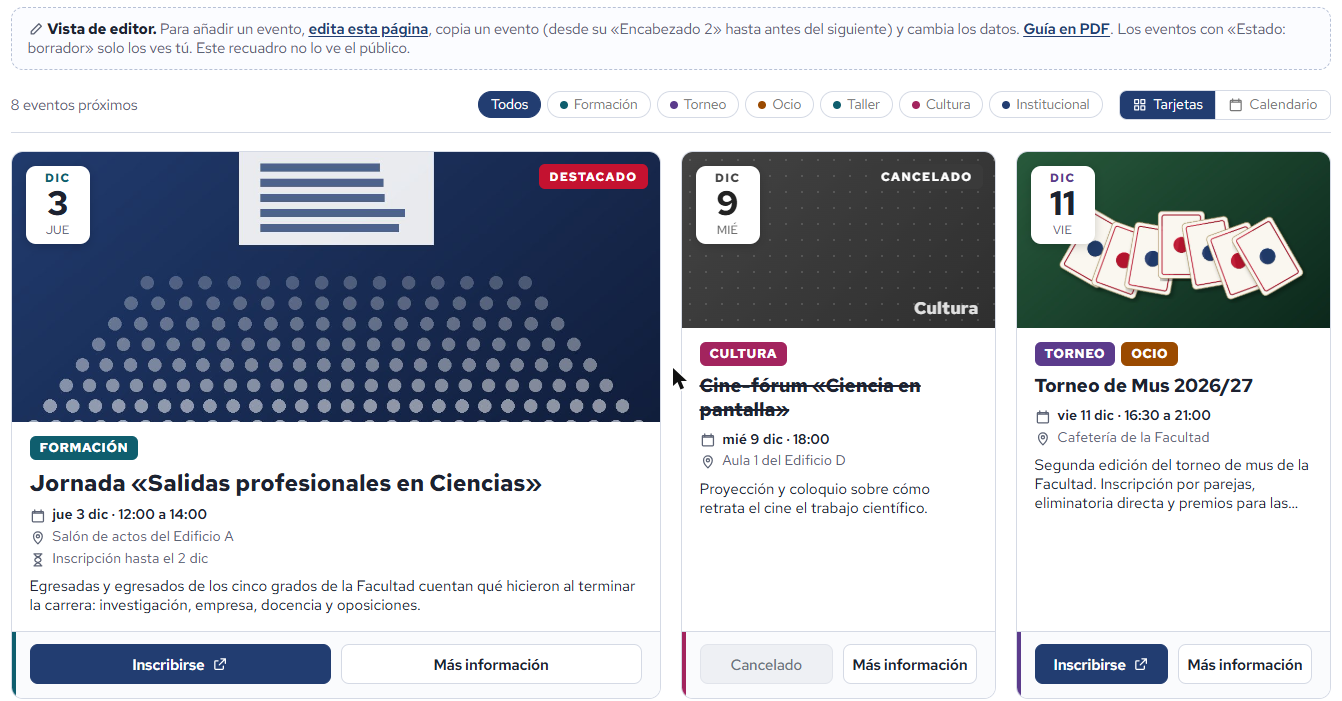
\includegraphics[width=\linewidth]{img/tarjetas.png}\\[2pt]
{\small\color{DarkGray3}Así se ve la página. El recuadro discontinuo de arriba solo aparece con la sesión iniciada.}
\end{center}

\section{Añadir un evento paso a paso}
\begin{enumerate}[leftmargin=*, itemsep=4pt]
  \item Entra en la web con tu cuenta de editor y abre \web{cienzdel.unizar.es/eventos}.
  \item Pulsa \boton{Editar}, en las pestañas que hay encima del título de la página (o el enlace
        «edita esta página» del recuadro de editor).
  \item Baja hasta el final del texto. El último evento se llama \textbf{«Plantilla para copiar»}:
        selecciónalo desde su título hasta su último párrafo, cópialo (\texttt{Ctrl+C}) y pégalo
        (\texttt{Ctrl+V}) justo encima de su título. El orden no importa: la página los ordena por fecha.
  \item Cambia el título y los datos de la copia (sección~\ref{sec:datos}).
  \item Deja la línea \textbf{«Estado: borrador»} de momento y pulsa \boton{Guardar} al final del formulario.
  \item Revisa el evento en la página: en borrador solo lo ven quienes tienen sesión iniciada, con un
        borde discontinuo. Si la página no entiende algo (una fecha mal escrita, por ejemplo), lo dice en
        el recuadro de editor.
  \item Cuando esté bien, vuelve a \boton{Editar}, borra la línea «Estado: borrador» y \boton{Guardar}.
        Ya es público.
\end{enumerate}

\begin{center}
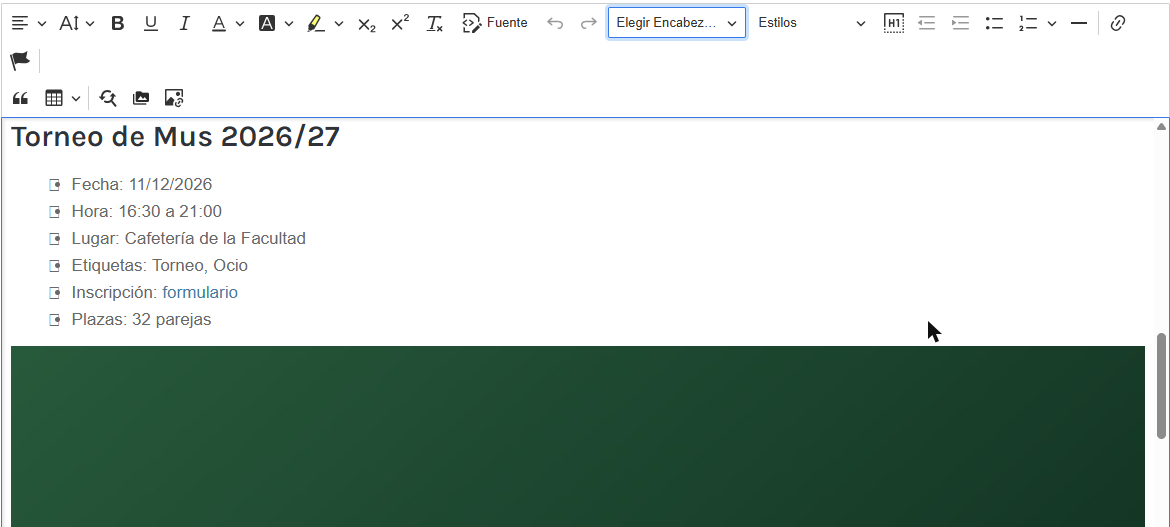
\includegraphics[width=0.92\linewidth]{img/editor.png}\\[2pt]
{\small\color{DarkGray3}Un evento en el editor de la web: título, lista de datos, imagen y párrafos.}
\end{center}

\begin{cuidado}[No borres estas dos cosas]
La página empieza con un bloque vacío y acaba con una línea de código invisible: son las que hacen
funcionar el tablón. No uses «Seleccionar todo» y «Suprimir», ni «Quitar formato» sobre toda la página.
La web no guarda versiones anteriores que un editor pueda recuperar, así que, antes de un cambio grande,
copia todo el texto a un documento aparte.

Si se borran, pulsa \boton{Fuente} en la barra del editor y escribe esta línea al principio del todo:
\begin{Verbatim}[fontsize=\footnotesize]
<div id="eventos-cienzdel"></div>
\end{Verbatim}
y esta otra al final del todo:
\begin{Verbatim}[fontsize=\footnotesize]
<script src="https://cienzdel.github.io/eventos/eventos.js"></script>
\end{Verbatim}
\end{cuidado}

\section{Cómo se escribe un evento}\label{sec:datos}
Un evento empieza en un \textbf{«Encabezado 2»} (el desplegable «Elegir Encabezado» de la barra del editor) y acaba
donde empieza el siguiente. Justo debajo del título va una \textbf{lista de viñetas} con una línea por dato,
siempre con la forma «Nombre: valor». Esto es lo que se escribe, tal cual:

\begin{tcolorbox}[colback=white, colframe=DarkGray3, boxrule=0.4pt, arc=1mm, left=3mm]
\textbf{\large Torneo de Mus 2026/27}\hfill{\small\color{DarkGray3}(Encabezado 2)}
\begin{itemize}[itemsep=0pt]
  \item Fecha: 11/12/2026
  \item Hora: 16:30 a 21:00
  \item Lugar: Cafetería de la Facultad
  \item Etiquetas: Torneo, Ocio
  \item Inscripción: \underline{formulario} {\small\color{DarkGray3}(con enlace al Google Forms)}
  \item Plazas: 32 parejas
\end{itemize}
{\small\color{DarkGray3}[imagen de portada]}\par
Segunda edición del torneo de mus de la Facultad. Inscripción por parejas…\par
Las partidas se juegan a 40 tantos, con ocho reyes…
\end{tcolorbox}

\subsection{Los datos que entiende la página}
\begin{tabularx}{\linewidth}{@{}>{\bfseries}l X@{}}
\toprule
Línea & Qué poner \\
\midrule
Fecha & Obligatoria. \texttt{11/12/2026}, «11 de diciembre de 2026» o, si dura varios días,
        «del 20 al 22 de enero de 2027». \\
Hora & \texttt{17:00}, «16:30 a 21:00» o «17 h». Opcional. \\
Lugar & Texto libre. Si le pones un enlace (por ejemplo, al aula en el visor del campus), se podrá pulsar. \\
Etiquetas & Separadas por comas: «Torneo, Ocio». Salen en grande en la tarjeta, con color, y sirven para
        filtrar. Usa las que ya existen (Formación, Taller, Torneo, Ocio, Institucional, Cultura, Deporte)
        para que los colores sean coherentes. La etiqueta especial \textbf{Destacado} no se muestra como
        etiqueta: pone la tarjeta al doble de ancho y un sello rojo. \\
Inscripción & Escribe una palabra («formulario»), selecciónala y ponle el enlace con \texttt{Ctrl+K}.
        Así aparece el botón \boton{Inscribirse}. Si no hay que inscribirse, escribe un texto sin enlace
        («no hace falta inscribirse») y saldrá en gris. Si no pones la línea, no sale botón. \\
Plazo & Último día para inscribirse: \texttt{10/12/2026}. Al día siguiente el botón pasa a
        «Inscripción cerrada». \\
Estado & \texttt{borrador} (solo lo ven los editores), \texttt{cancelado}, \texttt{aplazado} o
        \texttt{completo} (plazas agotadas). Sin esta línea, el evento es normal. \\
Otras & Cualquier otra línea con la forma «Nombre: valor» («Plazas: 32 parejas», «Trae: portátil»)
        se muestra tal cual en «Más información». \\
\bottomrule
\end{tabularx}

\subsection{El texto}
\begin{itemize}
  \item \textbf{El primer párrafo} después de la lista es el resumen de la tarjeta (unas tres líneas).
  \item \textbf{Todo lo demás} (párrafos, listas, «Encabezado 3», enlaces a reglamentos o a otras páginas)
        solo aparece al pulsar \boton{Más información}. Es como una noticia corta.
  \item \textbf{La primera imagen} del evento es la portada de la tarjeta. Ponla justo debajo de la lista
        con el botón del gestor de archivos (la carpeta con una foto, «Insert images using Imce File
        Manager»): en la ventana que se abre, sube el archivo, selecciónalo e insértalo. Después pulsa sobre
        la imagen y rellena su texto alternativo (qué se ve en ella). Lo mejor es un JPG apaisado de 1200\,×\,675 píxeles
        (proporción 16:9) y menos de 300\,kB. Sin imagen, la tarjeta usa el color de la primera etiqueta.
\end{itemize}

\section{El formulario de inscripción}
\begin{enumerate}[leftmargin=*]
  \item Crea el formulario en Google Forms con la cuenta del Consejo.
  \item Pulsa \boton{Enviar}, elige el icono del enlace, marca «Acortar URL» y copia el enlace
        (\texttt{forms.gle/…}).
  \item En la línea «Inscripción» de la web, selecciona la palabra «formulario», pulsa \texttt{Ctrl+K},
        pega el enlace y confirma.
  \item Cuando cierres el formulario en Google Forms, pon también el «Plazo» o «Estado: completo» en la
        web, para que el botón no lleve a un formulario cerrado.
\end{enumerate}

\begin{consejo}[Para la difusión]
En «Más información», el botón \boton{Copiar enlace} da la dirección directa del evento
(\texttt{cienzdel.unizar.es/eventos\#torneo-de-mus-2026-27}), que abre su ventana al entrar. Es la que
conviene poner en Instagram o en los correos. Ojo: depende del título, así que si lo cambias, cambia el enlace.
\end{consejo}

\section{Cambiar, cancelar o quitar un evento}
\begin{itemize}
  \item \textbf{Cambiar datos}: \boton{Editar}, cambia la línea que sea y \boton{Guardar}.
  \item \textbf{Cancelar}: añade «Estado: cancelado» y explica el motivo en el texto. La tarjeta se queda,
        tachada, para que quien se había apuntado lo vea.
  \item \textbf{Aplazar}: «Estado: aplazado» hasta que haya fecha nueva; entonces cambia la fecha y quita el estado.
  \item \textbf{Eventos pasados}: no hay que hacer nada. Al día siguiente pasan solos a «Eventos pasados»,
        al final de la página. Al acabar el curso se pueden borrar los del curso anterior.
\end{itemize}

\section{El calendario}
La pestaña \boton{Calendario} de la página muestra todos los eventos en una vista mensual (en el móvil,
como lista). Cada evento se puede añadir a Google Calendar o descargar como archivo \texttt{.ics} desde
su ventana.

Además, cualquiera puede suscribirse al calendario completo con los enlaces que hay debajo de la vista
mensual: el calendario se actualiza solo. Lo genera una tarea automática en
\web{github.com/cienzdel/eventos} que lee la página cada tres horas, así que un evento nuevo tarda como
mucho unas horas en llegar a los calendarios suscritos (en la web aparece al momento).

\section{Problemas frecuentes}
\begin{tabularx}{\linewidth}{@{}>{\raggedright\arraybackslash}p{0.36\linewidth} X@{}}
\toprule
Lo que pasa & Por qué y cómo se arregla \\
\midrule
El evento sale pegado al anterior, como texto suyo & El título no es «Encabezado 2» (quizá es «Encabezado 3»
  o un párrafo en negrita). Selecciónalo y elige «Encabezado 2» en «Elegir Encabezado». \\
«No encuentro la lista de datos» & Los datos no están en una lista de viñetas o les falta «Nombre:».
  Selecciona las líneas y pulsa el botón de lista de viñetas. \\
«No entiendo la fecha» & Escríbela como \texttt{11/12/2026} o «11 de diciembre de 2026». \\
No sale el botón «Inscribirse» & La palabra de la línea «Inscripción» no tiene enlace, o ya pasó el plazo. \\
La página se ve como texto plano & Se ha borrado la línea de código del final o el bloque vacío del
  principio. Vuelve a ponerlos con \boton{Fuente} (recuadro «No borres estas dos cosas»). \\
He cambiado algo y no se ve & Recarga la página. Si es un cambio del funcionamiento (no de un evento),
  puede tardar hasta diez minutos. \\
\bottomrule
\end{tabularx}

\vspace{6pt}
Dudas o sugerencias: \href{mailto:cienzdel@unizar.es}{cienzdel@unizar.es}. La explicación técnica está en
\web{github.com/cienzdel/eventos}.

\end{document}
